\documentclass{standalone}
\usepackage{tikz}
\usepackage{ctex,siunitx}
\setCJKmainfont{Noto Serif CJK SC}
\usepackage{tkz-euclide}
\usepackage{amsmath}
\usetikzlibrary{patterns, calc,3d}
\usetikzlibrary {decorations.pathmorphing,decorations.pathreplacing,decorations.shapes}
\tikzset{label style/.append style={font=\small}}
\begin{document}
\small
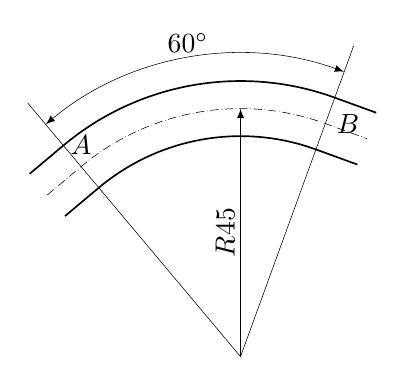
\begin{tikzpicture}[>=latex,scale=0.7,inner sep=2pt]
  \draw[very thin,densely dashdotted]([shift=(-140:0.8)]130:4.5)--(130:4.5)arc(130:70:4.5)--++(-20:0.8);
  \draw[semithick]([shift=(-140:0.8)]130:5)--(130:5)arc(130:70:5)--++(-20:0.8);
  \draw[semithick]([shift=(-140:0.8)]130:4)--(130:4)arc(130:70:4)--++(-20:0.8);
  \draw[very thin,->](0,0)--(90:4.5)node[midway,sloped,above]{$R45$};
  \draw[very thin](70:6)--(0,0)--(130:6);
  \node at (130:4.5)[above=2pt]{$A$};
  \node at (70:4.5)[right=2pt]{$B$};
  \draw[very thin,<->](130:5.5)arc(130:70:5.5)node[above,midway]{\ang{60}};
\end{tikzpicture}
\end{document}